%\title{Truncated Exponential Sampling}
%\author{Emanuel Casiano-Diaz}
%\date{January 19, 2022.}


%Formatting Packages
\documentclass[12pt, two sided]{article}
\usepackage[utf8]{inputenc}
%\usepackage[letter,top=1.1in,bottom=1.1in,left=1.6in,right=1.1in]{geometry}
\usepackage[letterpaper,margin=1in]{geometry}

\usepackage{graphicx}
\usepackage{subfig}
\usepackage{float}

%Math Packages
\usepackage{amsmath}
\usepackage{amssymb}
\usepackage{bm}
\DeclareMathOperator{\Tr}{Tr}

%Physics Package
\usepackage{physics}

%Allow accentuation marks
\usepackage[utf8]{inputenc}
\usepackage[T1]{fontenc}

%Image packages
\usepackage{graphicx}
\graphicspath{ {Images/} }

%Enumerating lists
\usepackage{enumerate}% http://ctan.org/pkg/enumerate

%Adjust depth of subsections
\setcounter{secnumdepth}{3}

%Adjust depth of table of contents
\setcounter{tocdepth}{3}

%References Packages
%\usepackage{biblatex}
%\addbibresource{references.bib}
\usepackage[bookmarks=true]{hyperref}
\hypersetup{
    hidelinks=true,
    linkcolor=blue,
    filecolor=magenta,      
    urlcolor=cyan,
}

%Commands and packages imported from particle entanglement paper
\usepackage{amsmath}
\usepackage{xcolor}
\usepackage{graphicx}
\usepackage{amssymb}

\newcommand{\eket}[1]{\bigl \vert #1 \bigr \rangle}
\newcommand{\R}{\boldsymbol{R}}
\newcommand{\Rt}{\tilde{\R}}
\newcommand{\ebra}[1]{\bigl \langle #1 \bigr \vert}
\newcommand{\eexp}[1]{\bigl \langle #1 \bigr \rangle}
\newcommand{\figref}[1]{Fig.~\ref{#1}}
\renewcommand{\vec}[1]{\boldsymbol{#1}}
\newcommand{\ren}{R\'{e}nyi~}
\newcommand{\rnote}[1]{{\it \textcolor{red}{#1} }}
\newcommand{\Eqref}[1]{Eq.~\eqref{#1}}

%Copied from paper
\usepackage{color}
\usepackage{graphicx}
\usepackage[color=green!60]{todonotes}
\usepackage{physics}
\usepackage{amsthm}
\usepackage{amsmath}
\usepackage{amssymb}
\usepackage{enumerate}
\usepackage{placeins}
\usepackage{booktabs}
\usepackage{dsfont}

%For reference formatting
\usepackage[numbers,sort&compress]{natbib}
\bibliographystyle{nsf_new_url}

\setlength{\footskip}{22pt}

 %Line spacing
\usepackage{setspace}
\doublespace

% --------- Begin Document -------- %
\begin{document}

%----- Introduction -------%


\section{Introduction}

In our $T=0$ Lattice Path Integral Monte Carlo code (insert hyperlink), the acceptance ratio each update usually involves an exponential factor. This factor comes in three forms:

\begin{itemize}
 \item Case 1: $\frac{W^\prime}{W} \propto e^{-c(\tau-a)} \;\;\;\;\;\;\; (a<\tau)$ \\
 \item Case 2: $\frac{W^\prime}{W} \propto e^{-c(b-\tau)} \;\;\;\;\;\;\; (b>\tau)$ \\
 \item Case 3: $\frac{W^\prime}{W} \propto e^{-c(\tau_2-\tau_1)} \;\;\;\;\; (a < \tau_1 < \tau_2 < b)$ 
 \end{itemize}

where $\tau$ is a previously sampled imaginary time, $a,b$ are lower and upper bounds of the sampling interval, respectively, and $c$ is a constant, that in practice turns out to be related to the energy difference between pre and post-update configurations. In the third case, two imaginary times $\tau_1, \tau_2$ are sampled subject to the constraint: $(a<\tau_1<\tau_2<b)$.

Before delving into the specifics of what the symbols will represent in the simulation, I would like to first establish the goal: cancelling these exponentials from the acceptance ratio. 

Recall that the acceptance ratio is given by:
%
\begin{equation}
R = \frac{W^\prime}{W} \frac{P}{P^\prime}
\end{equation}
%
where $W^\prime,W$ are the weights of worldline configurations, which for our algorithm is obtained from the path-integral formulation of the ground state weight, and $P,P^\prime$ are probabilities of proposing a certain update and can vary depending on the decision process we follow to propose the update. Primed quantities refer to post-update configurations, and unprimed ones refer to the configuration before the update. Since most updates involve the sampling of an imaginary time, we can choose to sample these times from distributions that look similar to the exponentials in the weight ratios. Strategically choosing from what distribution to sample from, can change the proposal probability ratios $P/P^\prime$, such that the exponentials in the weight ratios cancel.

We will discuss some examples that illustrate how to sample in each of the cases above. 

%-----------------------------   Case 1 ----------------------------------------------%
\section{Case: $P(\tau) \propto e^{-c(\tau-a)}$}

Some of the updates in out Lattice PIMC algorithm will have an acceptance ratio of the form:

\begin{equation}
R =  \frac{W^\prime}{W} \frac{P}{P^\prime} = Ae^{-c(\tau-a)} \frac{P}{P^\prime}
\end{equation}

where $a<\tau$. A is just a constant (or actually product of constants that is obtained from the weight ratio calculation). In order to cancel the exponential factor coming from the weights, the proposal probability ratio needs to be of the form:

\begin{equation}
\frac{P}{P^\prime} = \frac{B}{\frac{c}{\mathcal{Z}}e^{-c(\tau-a)}}
\end{equation}

where $B$ is in general a product of probabilities dependent on how the update is proposed, and the prefactor $1/\mathcal{Z}$a normalizes the distribution. As part of most updates, an imaginary time $\tau$ needs to be proposed or sampled, and we will sample it from what is known as a truncated exponential distribution:

\begin{equation}
P^\prime \equiv P(\tau) = \frac{c}{\mathcal{Z}}e^{-c(\tau-a)}
\end{equation}

From now on, we can be quite methodic. A random variate $\tau$ can be obtained from $P(\tau)$ by: 1) Computing the normalization constant, 2) Computing the cumulutaive distribution function as a function of the random variate, and 3) inverting the cdf.

To normalize $P(\tau)$, integrate over all possible values of $\tau$ and equate to unity:

\begin{align}
1 &= \frac{c}{\mathcal{Z}} \int_{a}^{b} e^{-c(\tau-a)} d\tau \\
&= \frac{c}{\mathcal{Z}} e^{ca} \int_{a}^{b} e^{-c\tau} d\tau \\
&= \frac{c}{\mathcal{Z}} e^{ca} [-\frac{1}{c}] [e^{-cb}-e^{-ca}] \\
&= -\frac{1}{\mathcal{Z}} [e^{-c(b-a)}-1] \\
&= \frac{1}{\mathcal{Z}} [1-e^{-c(b-a)}] \\
\end{align}

Solving for $\mathcal{Z}$, the normalization constant becomes:

\begin{equation}
\mathcal{Z} = 1 - e^{-c(b-a)}
\end{equation}

The next to step is to compute the cumulative distribution function (CDF) and equate it to a uniformly distributed random number $x\in[0,1)$:

\begin{equation}
x \equiv \frac{c}{\mathcal{Z}} \int_{a}^{\tau} e^{-c(\tau^\prime-a)} d\tau\prime = \frac{1}{\mathcal{Z}}[1-e^{-c(\tau-a)}]
\end{equation}

Finally, solving for the random time $\tau$, we obtain:

\begin{equation}
\tau = a - \frac{1}{c} \ln(1-\mathcal{Z}x)
\end{equation}

Sampling $\tau$ from this distribution leads to an acceptance ratio that has the form:

\begin{align}
R &= \frac{W^\prime}{W} \frac{P}{P^\prime} \\
&= A e^{-c(\tau-a)} \frac{B}{\frac{c}{\mathcal{Z}}e^{-c(\tau-a)}} \\
R &= \frac{A B \mathcal{Z}}{c} 
\end{align}

The original exponential coming from the weight ratio has been cancelled. The idea is that since the acceptance ratio $R$ only involves constants now, and no random variates, simulation parameters, such as the fugacity $\eta$, could be smartly equilibrated to obtain a desired acceptance ratio, that should be roughly constant, independent of the random time sampled. This might in turn enhance the dynamics of the worldline configuration and reduce autocorrelation and numbers of samples needed to achieve convergence of an estimator.

%-----------------------------   Case 2 ----------------------------------------------% 

\section{Case: $P(\tau) \propto e^{-c(b-\tau)}$}

Some other updates will have an acceptance ratio of the form
\begin{equation}
R =  \frac{W^\prime}{W} \frac{P}{P^\prime} = Ae^{-c(b-\tau)} \frac{P}{P^\prime}
\end{equation}

where $b>\tau$. Note that exponential coming from the weight ratio now depends on $b$, which is the upper bound of the interval, rather than $a$, which is the lower bound. Additionally, there is a sign of the random variate $\tau$, which is now negative, and $b$ is positive. The process follows the same steps as case 1, but we now sample $\tau$ instead from the following distribution:

\begin{equation}
P^\prime \equiv P(\tau) = \frac{c}{\mathcal{Z}}e^{-c(b-\tau)}
\end{equation}

where the normalization constant is left unchanged. The CDF is obtained almost the same way as before, but the limits of integration go from $\tau$, the random time, to $b$, the upper bound:

\begin{equation}
x \equiv \frac{c}{\mathcal{Z}} \int_{\tau}^{b} e^{-c(b-\tau^\prime)} d\tau\prime = \frac{1}{\mathcal{Z}}[e^{-c(b-\tau)}]
\end{equation}

and again, solving for $\tau$ gives us the random imaginary time sampled from a truncated exponential distribution:

\begin{equation}
\tau = b + \frac{1}{c} \ln(1-\mathcal{Z}x)
\end{equation}

which cancels the exponential coming from the weight ratio, when computing the acceptance ratio $R$:

\begin{align}
R &= \frac{W^\prime}{W} \frac{P}{P^\prime} \\
&= A e^{-c(b-\tau)} \frac{B}{\frac{c}{\mathcal{Z}}e^{-c(b-\tau)}} \\
R &= \frac{A B \mathcal{Z}}{c} 
\end{align}

%-----------------------------   Case 3 ----------------------------------------------% 

\section{Case: $P(\tau) \propto e^{-c(\tau_2-\tau_1)}$}

The final case is that in which the weight ratio depends on not one, but two random variates $\tau_1,\tau_2$. In the discussion that follows, we will assume that the random times follow are subject to the constraint: $ a < \tau_1 < \tau_2 < b $. A prototypical acceptance ratio for this case has the following form:

\begin{equation}
R =  \frac{W^\prime}{W} \frac{P}{P^\prime} = A e^{-c(\tau_2-\tau_1)} \frac{P}{P^\prime}
\end{equation}

As such, as part of the decision process followed to build the proposal probability ratio, it will be wise to sample the imaginary times from the following joint probability distribution:

\begin{equation}
P^\prime \equiv P(\tau_1,\tau_2) = \frac{c}{\mathcal{Z}} e^{-c(\tau_2-\tau_1)}
\end{equation}

In practice, we don't sample the two times simultaneously, but one at a time, rather. To do this, we will employ the following property of joint probability distributions:

\begin{equation}
P(\tau_1,\tau_2) = P(\tau_1) P(\tau_2 \vert \tau_1)
\end{equation}

where $P(\tau_1)$ is the marginalized probability of $\tau_1$, obtained by integrating out the $\tau_2$ dependence. The factor $P(\tau_2 \vert \tau_1)$ is the probability of sampling $\tau_2$, conditional on the value of $\tau_1$. The strategy we will follow is to first sample $\tau_1$ from $P(\tau_1)$ and then $\tau_2$ from $P(\tau_2 \vert \tau_1)$.

Integrating out the $\tau_2$ dependence, the marginalized probability distribution of $\tau_1$ can be obtained:

\begin{align}
P(\tau_1) &= \int_{\tau_1}^{b} P(\tau_1,\tau_2) d\tau_2 \\
&= \frac{c}{\mathcal{Z_1}} \int_{\tau_1}^{b} e^{-c(\tau_2-\tau_1)} d\tau_2 \\
&= \frac{c}{\mathcal{Z_1}} e^{c\tau_1} \int_{\tau_1}^{b} e^{-c\tau_2} d\tau_2 \\
&= -\frac{1}{\mathcal{Z_1}} e^{c\tau_1} [e^{-cb}-e^{-c\tau_1}] \\
&= -\frac{1}{\mathcal{Z_1}} e^{c\tau_1} [e^{-cb}-e^{-c\tau_1}] \\
P(\tau_1) &= \frac{1}{\mathcal{Z}}  [1-e^{-c(b-\tau_1)}] \\
\end{align}

Where $Z_1$ is the normalization constant of the marginalized distribution $P(\tau_1)$, and the original constant $\mathcal{Z}$, corresponding to the joint distribution has been absorbed by it. Since now both the joint and the marginalized distributions are known, the conditional distribution can be solved for from the property shown above:

\begin{align}
P(\tau_2 \vert \tau_1) &= \frac{P(\tau_1,\tau_2)}{P(\tau_1)} \\
&\propto c \frac{\mathcal{Z_1}}{\mathcal{Z}} \frac{e^{-c(\tau_2-\tau_1)}}{1-e^{-c(b-\tau_1)}} \\
P(\tau_2 \vert \tau_1) &= \frac{c}{\mathcal{Z_2}} e^{-c(\tau_2-\tau_1)}
\end{align}

Since in the expression above, $\tau_1$ is assumed to have already been sampled, it can be treated as a constant. Moreover, all other constants have been absorbed into the normalization constant $Z_2$, corresponding to the conditional distribution, except $c$ since the benefit of hindsight tells us that we can leave it there to be cancelled after the $Z_2$ is explicitly computed. Note that the conditional probability is just a simple truncated exponential distribution like the one discussed in case 1.

We are now almost there. Distributions have been computed that will allow for the sampling of $\tau_1$ and then $\tau_2$, such that they effectively are sampled from the joint distribution. The rest from now on follows the same process as the previous cases: computing the normalization constant, the cdf, and the form of the random variates.

For the marginalized distribution, the normalization constant gives:

\begin{align}
1 &= \frac{1}{\mathcal{Z_1}} \int_{a}^{b} [ 1-e^{-c(b-\tau_1)} ] d\tau_1\\
1 &= \frac{1}{\mathcal{c Z_1}} [e^{-c(b-a)}+c(b-a)-1]
\end{align}

and the normalization constant becomes:

\begin{equation}
\mathcal{Z_1} = \frac{1}{c} [e^{-c(b-a)}+c(b-a)-1]
\end{equation}

The cdf is: 

\begin{align}
x &= \frac{1}{\mathcal{Z_1}} \int_{a}^{\tau_1} [ 1-e^{-c(b-\tau^{\prime}_1)} ] d\tau^{\prime}_1\\
x &= \frac{1}{\mathcal{Z_1}} [\tau_1 - a + \frac{1}{c} (e^{-c(b-a)}-e^{-c(b-\tau_1)})] \\
\end{align}

Solving for $\tau_1$ can get slightly tricky here. First, try leaving all $\tau_1$ dependence to one side of the equation:

\begin{equation}
\mathcal{Z_1} x + a - \frac{1}{c} e^{-c(b-a)} = \tau_1 - \frac{1}{c} e^{-c(b-\tau_1)}
\end{equation}

perform the following substitutions for simplicity:

\begin{equation}
y = \mathcal{Z_1} x + a - \frac{1}{c} e^{-c(b-a)}
\end{equation}

\begin{equation}
A = \frac{1}{c} e^{-cb}
\end{equation}

and the equation becomes:

\begin{equation}
y = \tau_1 - A e^{c \tau_1}
\end{equation}

which, solving for $\tau_1$, has the solution:

\begin{equation}
\tau_1 = y - \frac{1}{c} W_{k}(-Ac e^{cy})
\end{equation}

where $W_{k}$ is the Lambert-W or Product Log function and $k\in\mathbb{Z}$. 

From here on, the process for sampling $\tau_2$ follows the same steps as Case 1, but replacing $a=\tau_1$ in the exponent and $\tau_2=\tau$.

By sampling $\tau_1$ and then $\tau_2$ as prescribed, we have effectively sampled from the joint probability distribution $P(\tau_1,\tau_2)$. Finally, let's take a look at the effect of sampling from these joint distribution on the acceptance ratio:

\begin{align}
R &= \frac{W^\prime}{W} \frac{P}{P^\prime} \\
&= A e^{-c(\tau_2-\tau_1)} \frac{B}{\frac{c}{\mathcal{Z}}e^{-c(\tau_2-\tau_1)}} \\
R &= \frac{A B \mathcal{Z}}{c} 
\end{align}

where the normalization of the joint distribution is:

\begin{equation}
\mathcal{Z} = \frac{1}{c^2} [e^{-c(b-a)}+c(b-a)-1]
\end{equation}

In the following section, example distributions will be shown built from sampling random variates in each of the three cases.

%-----------------------------   Sampling examples ----------------------------------------------% 

\section{Sampling examples}

\subsection{$P(\tau) \propto e^{-c(b-\tau)}$}

Parameters: $ c=-3.14 , a = 0.5, b = 1.4$

\begin{figure}[h!]
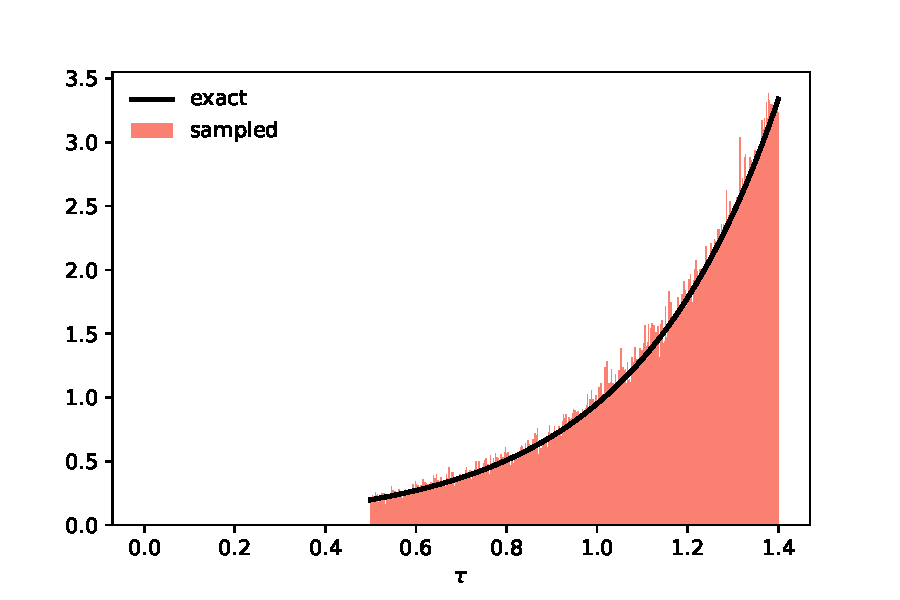
\includegraphics[width=8cm]{Figures/case1_cneg.pdf}
\end{figure}

Parameters: $ c=+3.14 , a = 0.5, b = 1.4$

\begin{figure}[h!]
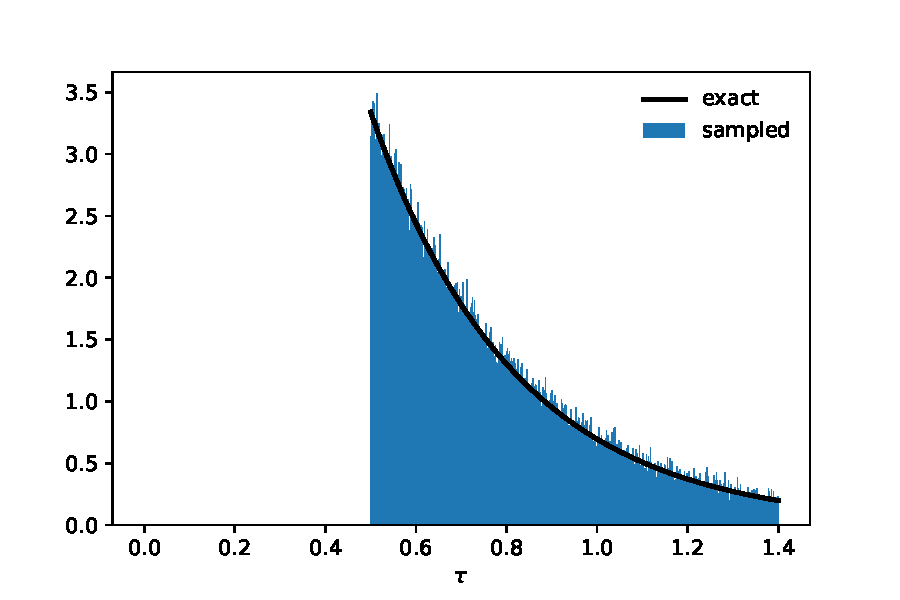
\includegraphics[width=8cm]{Figures/case1_cpos.pdf}
\end{figure}

\subsection{$P(\tau) \propto e^{-c(b-\tau)}$}

Parameters: $ c=-3.14 , a = 0.5, b = 1.4$

\begin{figure}[h!]
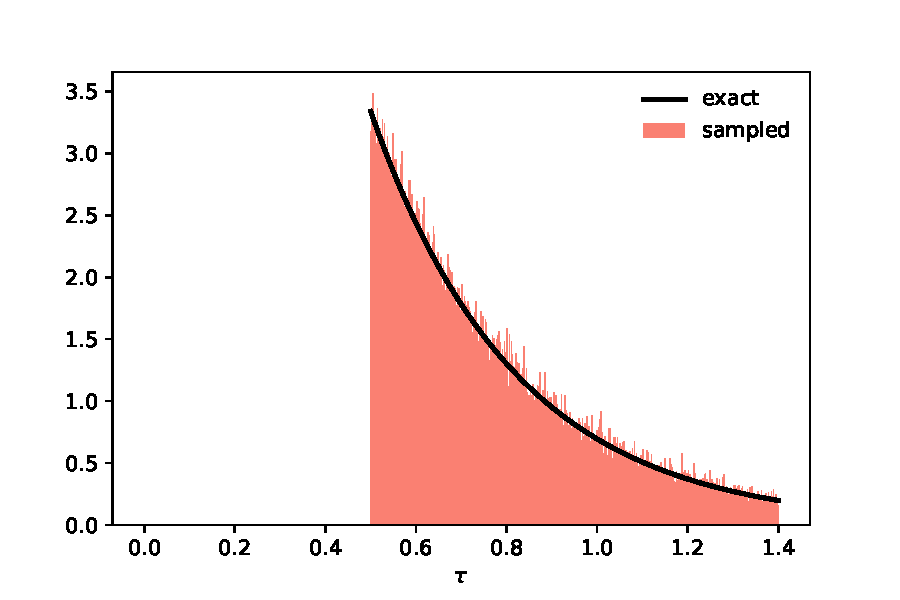
\includegraphics[width=8cm]{Figures/case2_cneg.pdf}
\end{figure}

Parameters: $ c=+3.14 , a = 0.5, b = 1.4$

\begin{figure}[h!]
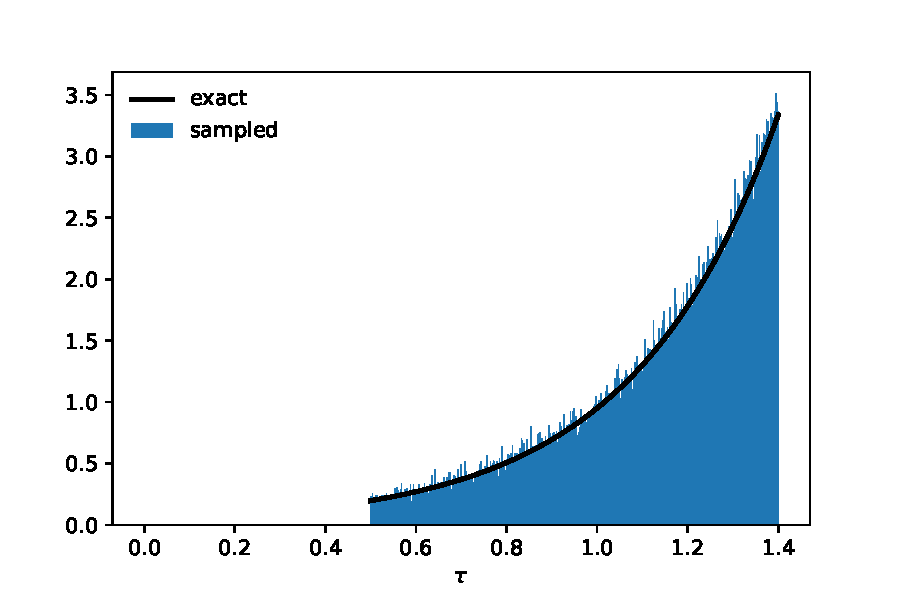
\includegraphics[width=8cm]{Figures/case2_cpos.pdf}
\end{figure}

\subsection{$P(\tau) \propto e^{-c(b-\tau)}$}

$ c=-0.5 , a = 0.1, b = 1.3 $

\begin{figure}[h!]
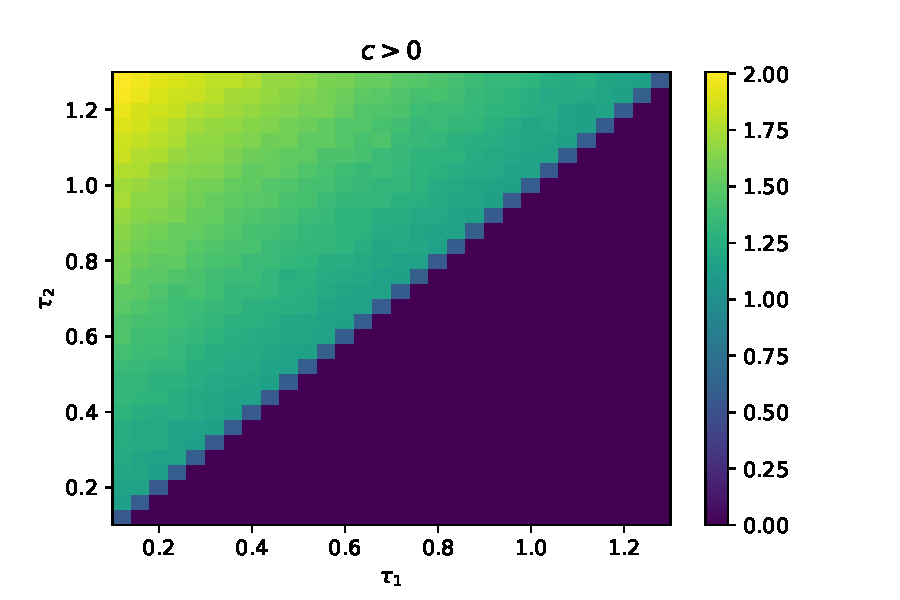
\includegraphics[width=8cm]{Figures/0.100000_1.300000_0.500000_sampled.pdf}
\end{figure}

Relative error:

\begin{figure}[h!]
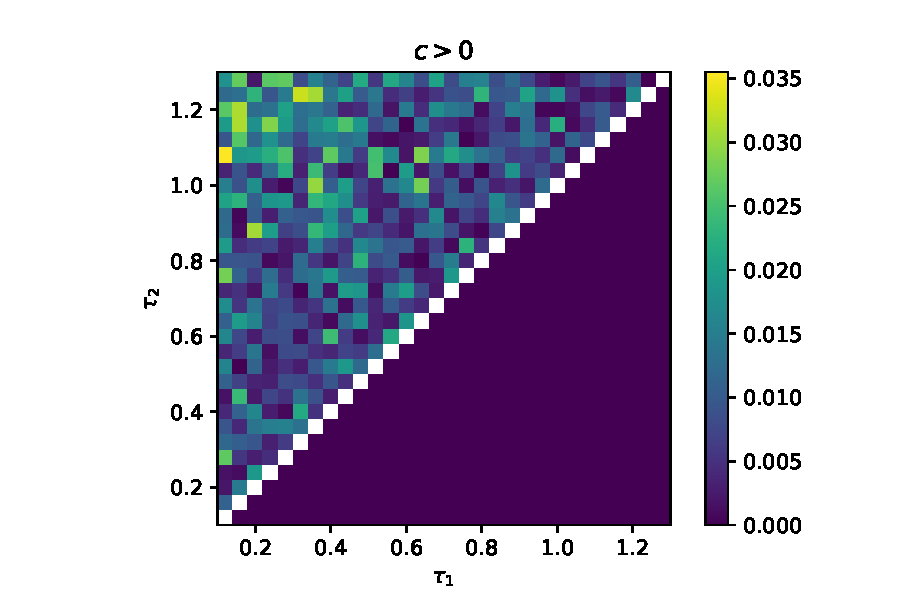
\includegraphics[width=8cm]{Figures/0.100000_1.300000_0.500000_relativeError_masked.pdf}
\end{figure}

$ c=0.5 , a = 0.1, b = 1.3 $

\begin{figure}[h!]
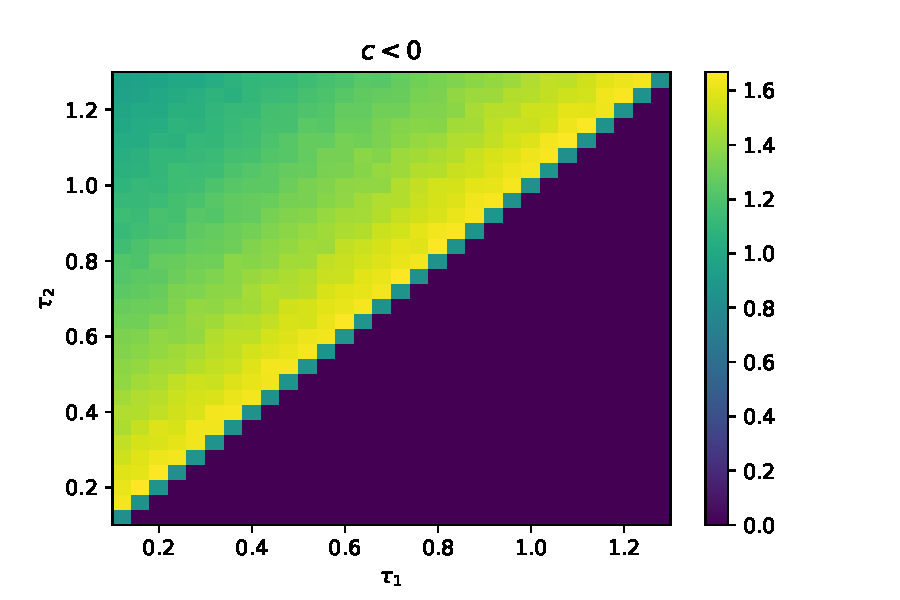
\includegraphics[width=8cm]{Figures/0.100000_1.300000_-0.500000_sampled.pdf}
\end{figure}

Relative error:

\begin{figure}[h!]
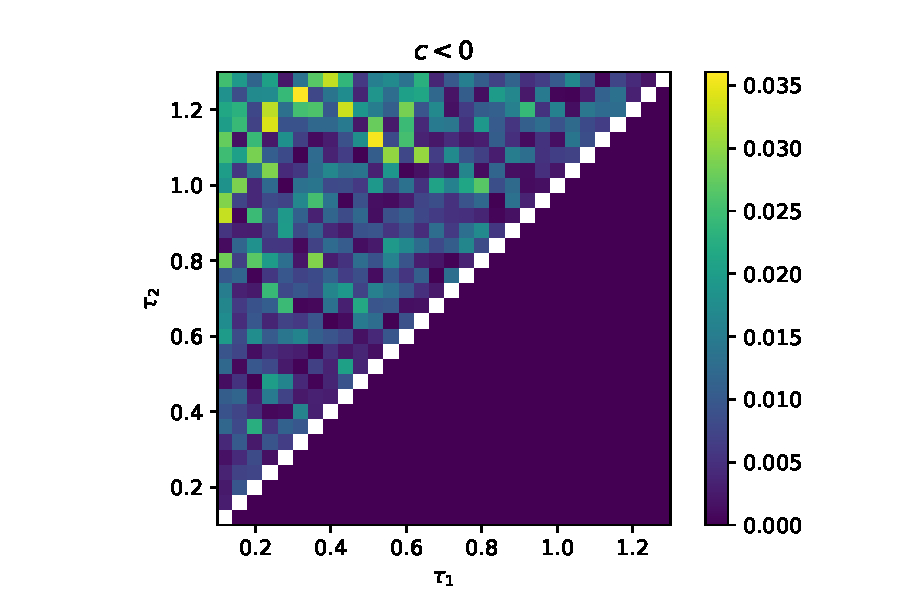
\includegraphics[width=8cm]{Figures/0.100000_1.300000_-0.500000_relativeError_masked.pdf}
\end{figure}

%-----------------------------   Energy benchmark ----------------------------------------------% 

\section{Energy benchmark}

Energy benchmark for $N=4$ particles, at unit filling, with $U/t=3.3$:

Kinetic:
\begin{figure}[h!]
\includegraphics[width=8cm]{Figures/runningAve_K_truncated.pdf}
\end{figure}

Potential:

\begin{figure}[h!]
\includegraphics[width=8cm]{Figures/runningAve_V_truncated.pdf}
\end{figure}

Truncated sampling:

\begin{table}[h!]
\begin{tabular}{lllll}
 $\langle K \rangle$ &  $-7.0322$ &  $-7.0378 \pm 0.0132$ & $0.4254\sigma$  \\
 $\langle V \rangle$ & $2.5490$ & $2.5482 \pm 0.0104$  & $0.0710\sigma$\\
\end{tabular}
\end{table}

Uniform sampling:

\begin{table}[h!]
\begin{tabular}{lllll}
 $\langle K \rangle$ &  $-7.0322$ &  $-7.0447 \pm 0.0126$ & $0.9953\sigma$  \\
 $\langle V \rangle$ & $2.5490$ & $2.5446 \pm 0.0089$  & $0.4919\sigma$\\
\end{tabular}
\end{table}

%-----------------------------   Wall clock and Autocorrelation times ----------------------------------------------% 

\section{Wall clock and Autocorrelation times}

In this section, a comparison will be made between the performance of the code using the truncated exponential sampling proposed here, and the original version of the code, which used mostly uniform sampling for the updates. For this comparison, the kinetic energy and the potential energy will be computed for a system using each sampling method. Then, the runtime of the code and the autocorrelation time will be computed for each. The simulation parameters can be read off from the command-line call:

 %./pigsl.e -D 1 -L 20 -N 20 -l 10 -U 3.300000 --mu 0.314159 --subgeometry square --measurement-frequency 1 --rng boost_mt19937 --bin-size 1 --bins-wanted 20000 --sweeps 1000000 --num-replicas 1 --beta 4.0 --seed 1968 --canonical --num-replicas 1 --no-accessible

The run times for 20 particles and for each method were:

\textbf{Truncated: $t = 68.03$ seconds and $t = 229.89$ seconds (4 times more bins)}

\textbf{Uniform: $t = 67.43$ seconds and $t = 230.14$ seconds (4 times more bins)}

Where the first time corresponds to generating 20000 bins and the second, 80000 bins.

Since the actual runtime was more or less the same for both runs, we now take a look at the autocorrelation time. This quantity gives an estimate of how correlated the samples are. Data with a smaller autocorrelation time becomes decorrelated more quickly and less samples need to be stored to obtain as good statistics as those obtained from more correlated data.

Kinetic energy (truncated):

\begin{figure}[h!]
\includegraphics[width=8cm]{Figures/Act_kinetic_truncated.pdf}
\end{figure}

Kinetic energy (truncated):

\begin{figure}[h!]
\includegraphics[width=8cm]{Figures/Act_kinetic_truncated.pdf}
\end{figure}

\textbf{Truncated: $act = 106.02$ Uniform: $act = 158.35$}

Potential energy (uniform):

\begin{figure}[h!]
\includegraphics[width=8cm]{Figures/Act_kinetic_uniform.pdf}
\end{figure}

Potential energy (uniform):

\begin{figure}[h!]
\includegraphics[width=8cm]{Figures/Act_kinetic_uniform.pdf}
\end{figure}

\textbf{Truncated: $act = 151.75$ Uniform: $act = 199.69$}


% ------------------------------------------------------ end ---------------------------------- %

% References
\phantomsection 
\addcontentsline{toc}{chapter}{References} 
%\bibliographystyle{apalike} %acm, ieetr, apalike...
 %\section*{Referencess
 \singlespacing
\bibliography{references}

\doublespacing

\end{document}
